\documentclass{llncs}
\usepackage{graphicx}
\usepackage{placeins}
\usepackage{upgreek}
\usepackage{amsmath}
\usepackage{subfig}
%
\begin{document}
\pagestyle{headings} 
\mainmatter
%
\title{Hybrid Approach Based on Combination of Backpropagation and Evolutionary Algorithms for Artificial Neural Networks Training by Using Mobile Devices in Distributed Computing Environment}
%
\author{Iliyan Zankinski, Maria Barova, Petar Tomov}
%
\authorrunning{Iliyan Zankinski} 
%
\tocauthor{Iliyan Zankinski, Maria Barova, Petar Tomov}
%
\institute{Institute of Information and Communication Technologies\\
Bulgarian Academy of Sciences\\
acad. G. Bonchev Str, Block 2, 1113 Sofia, Bulgaria\\
\email{iliyan@hsi.iccs.bas.bg}}
%
%Iliyan Zankinski iliyan@hsi.iccs.bas.bg
%Maria Barova m.barova@iit.bas.bg
%Petar Tomov p.tomov@iit.bas.bg 
%
\maketitle
%
\begin{abstract}
When Evolutionary Algorithms (EAs) are used for Artificial Neural Networks (ANNs) training, the most valuable advantage is the potential for this training to be done in parallel or even using distributed computing. With the capabilities of modern mobile devices, for example their use for distributed computations, they can be used much more extensively for scientific calculations. It is well known that distributed computing systems are limited by their communication bandwidth, because of network latency. In such environment some EAs are pretty suitable for distributed implementation. This is because of their high level of parallelism and relatively less intensive network communication needs. Subset of distributed computing is volunteer computing where users donate some of the computing power provided by devices under their control. This research proposes Android Live Wallpaper volunteer computing implementation of a system used for financial time series prediction. The forecasting module is organized as ANN, which is trained by hybrid combination of Backpropagation and EAs. 
\keywords{Artificial Neural Networks, Evolutionary Algorithms, Distributed Computing}
\end{abstract}
%
\section{Introduction}
%
ANNs are very common in the field of machine learning. In its nature ANN training is an optimization problem. When the searching space is too big, global optimization EAs as Genetic Algorithms (GAs) can be very suitable. In the last two decades there are numerous attempts to combine EAs based optimization with ANNs training. This combination shows to be much more promising when it is implemented as distributed computing system [1,2,3]. With the rising popularity of mobile devices a lot of new possibilities for distributed computing can be investigated. Successful desktop distributed computing projects, as described in [4,5] can be efficiently implemented on mobile devices. This idea can be applied to EA based ANN training into a mobile distributed computing environment [6]. In this paper a genetic algorithm in combination with backpropagation artificial neural network training is described. The training is done on a mobile devices as active Android wallpaper application. In addition, the traditional ANN's sigmoid function is replaced by fading sinusoidal function. The successful application of this hybrid approach is documented by series of experiments.

This paper is organized as follows. Section 1 gives an overview of the problem  with a special emphasis on ANNs/GAs and their strengths/weaknesses when applied for the problem's solution. Section 2 introduces a distributed computing system based on mobile devices. Experiments and results are presented in Section 3. The final Section 4 concludes and some further work suggestions are provided. 
%
\subsection{Financial Time Series Forecasting}
%
A time series is a collection of measurements made in a sequence through time. There are many examples for time series like the sales of the specific stock in successive months, the average daily temperature at a particular location, the electricity consumption in a particular areal for successive seasons and many other. In the field of the finance, decision makers are in the position of taking very responsible steps during formation of investment strategy. To invest it means to take acceptable risk with expectation of certain amount of profit. The most important aspect of investment is the balance between risk taken and expected profit. On the currency market (FOREX) the main trading is done by exchanging currencies. Currency is the most volatile in price changing object of trading. During the process of trading on a market as FOREX decision makers needs to take three important decisions: 1. Price will go up or down; 2. What volume to buy or sell; 3. How long to keep the opened position. Even if it sounds simple in fact it is very difficult to estimate price changing direction, because of the huge number of factors influencing it. The order volume is directly related to the amount of risk taken. High volume order can lead to high profit if price changing direction is well estimated, but it can lead to high loss in the other case. How long to keep the opened position is related to making the profit even bigger or making the loss as small as possible. Financial forecasting is most important for the traders on the currency market, because of the high price dynamics [2].
%
\subsection{Artificial Neural Networks}
%
Artificial Neural Network is a mathematical model inspired by research into the nature of the human brain. ANNs consists of five components: 

1. Network topology which is represented by a directed graph where arcs are referred as links.

2. A variable which represents the state of each node.

3. For each link a real value variable represents its weight.

4. A real value bias which is supplied to each node.

5. Node transfer function which determines the state of the node. The transfer function consists of an activation function (in most cases sigmoid or hyperbolic tangent). The activation function accepts the sum of the inputs multiplied by the weights of the links between the node and the input nodes.

When the network type is feed-forward there is no recurrent links (graph without loops). The input nodes in such network do not have input arcs. In order for the network to process information the input nodes should be supplied with values. After that the input information can be spread across the network. This action is known as feed-forward pass and it means that the other nodes are changing their state variable according to the propagation rules. The most used ANN topology is multilayer perceptron (MLP). In such network any path from an input node to an output node traverses the same number of arcs. A hidden layer in such ANN is a group of nodes which are neither input nor output and are on the same number of arcs distance from the input layer and the output layer. The network is fully connected if each node in a particular layer is connected to each node in the previous layer. 

MLP is so popular because of several reasons. Research shows that such networks generalize well in practical problems. When trained on a relatively sparse set of data points, they often provide the right output for an input not presented in the training set. Secondly, gradient based training algorithms like backpropagation of errors can be successfully applied in order to find a good set of weights in acceptable amount of time. The advantage of backpropagation is in calculating the gradient of the error according to the weights for a given input by back propagating the error through the network. Of course there are some disadvantages in gradient based training algorithms. Gradient based training works well on simple training problems. When the problem complexity increases (most commonly because of the increased dimensionality and/or greater data complexity) the performance of the gradient based training falls off rapidly. 

The performance slow down seems to come from the fact that complex spaces have nearly global optimum around the local optimum. Gradient search techniques tend to get trapped at the local optimum. With a high enough gain (or momentum), backpropagation can escape these local optima. However, it leaves them without knowing whether the next one it finds will be better or worse. When the nearly global optima are well hidden among the local optimum, backpropagation can end up bouncing between local optima without much overall improvement, thus making for very slow training. The second drawback of the gradient based training is the requirement for the activation function differentiability. Backpropagation can not handle discontinuous functions or discontinuous node activation functions.
%
\subsection{Genetic Algorithms}
%
Genetic Algorithms are meta heuristics for global optimization inspired from the ideas of biological evolution. They have five components:

1. Approach for encoding the problem in terms of chromosomes (population of individuals).

2. An evaluation function which is used to determine survival capabilities of each chromosome.

3. A strategy for initial population initialization.

4. Set of operator applied over parent chromosomes in order reproduction to appear (in most cases – selection, crossover, mutation and/or domain specific genetic material recombination).

5. Set of parameters applied over the population and the operators.

\vspace{4 mm}

GA applies these components and operates in the following steps:

1. Initialization of the population (can be random or according some prior information).

2. Evaluation of each chromosome in the population. Relative ranking is the important result in this step.

3. Epochs of recombinations are executed until stopping criteria is met.

  \hspace{4 mm}3.1 Parents selection is generally stochastic but parents with better fitness value are preferred.
  
  \hspace{4 mm}3.2 Recombination operators are applied over the selected parents in order to produce children.
  
  \hspace{4 mm}3.3 Evaluation of the children is done in order to keep some of them in the population. In some cases the whole old population is replaced by the new generation, but in other cases only part of the new generation is kept. The elitism rule is applied by keeping the best found individuals to survive until the end of the evolution.

If appropriate problem encoding and recombination operators are selected the algorithm is capable of producing better and better solutions, converging finally on results close to a global optimum. In most of the real life problems (as the problem presented in this research) standard operators as crossover and mutation are sufficient. In this case GA can be used as black-box optimizer. It means that no specific knowledge of the problem domain is needed. As it is shown in this research by involving problem specific operators (crossover and mutation), the optimization efficiency can be improved. 

GA does not have a scaling problem as it is the case with ANN. Even more, GAs are very suitable for parallel computing and even for distributed computing. This is the case because GA improves the current best candidate monotonically. It is done by keeping the best found candidates as part of the population while searching for better candidates continues. GAs are not threatened by getting stuck in a local optimum. The mutation and crossover operators can step from a valley across a hill to an even lower valley with no more difficulty than descending directly into a valley.
%
\subsection{Neuron Activation Function Proposal}
%
The most often used activation functions in MLPs are the sigmoid function and the hyperbolic tangent function [7]. In this research sin function with exponent fading effect is proposed as neurons activation function (Fig. 1). Because of its fading effect neurons are more active in a specific input range. If the input is highly positive or highly negative the neuron stops acting as effect of over saturation.
%
\begin{equation}
f(x) = \frac {\pi \sin(x)} { e^{ |x| }}
\end{equation}
%
The proposed function (Eq. 1) is differentiable (Eq. 2, Eq. 3) which is one of the common requirements in gradient based training of ANNs.
%
\begin{figure}
    \centering
    \subfloat[Function]{{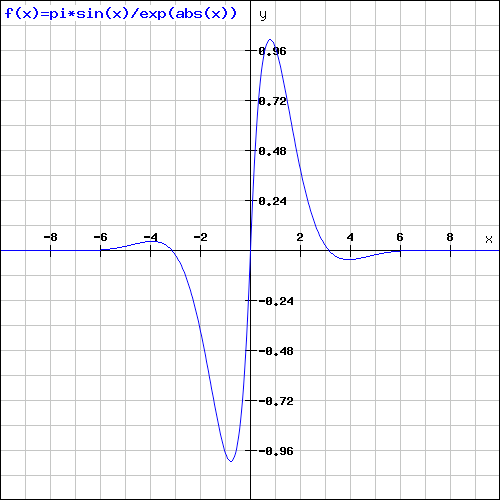
\includegraphics[width=6cm,height=6cm]{fig03.png} }}
    \subfloat[Derivative]{{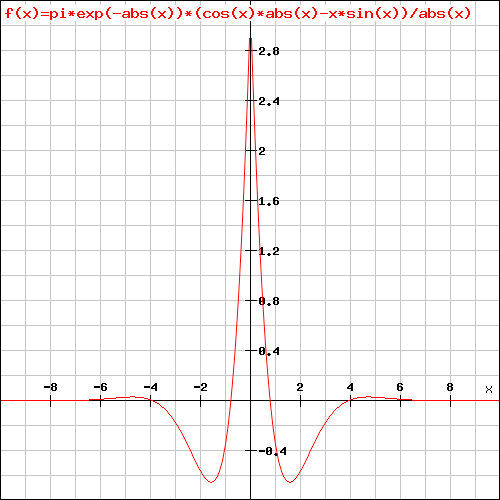
\includegraphics[width=6cm,height=6cm]{fig04.png} }}
    \caption{Exponent regulated sin activation function and its derivative.}
    \label{fig:fig01}
\end{figure}
\FloatBarrier
%
\begin{equation}
\frac{d}{dx}f(x) = \frac {\pi (|x|\cos x - x\sin x)} { |x| e^{ |x| } }
\end{equation}
%
Function derivative can be expressed by the function itself as it is shown in Eq. 3.
%
\begin{equation}
\frac{d}{dx}f(x) = 
\left\{
	\begin{array}{ll}
		f(x + \pi) - f(x) & \mbox{, } x > 0 \\
		f(x + \pi) + f(x) & \mbox{, } x < 0 \\
		+\infty & \mbox{, } x = 0
	\end{array}
\right.
\end{equation}
%
The advantage of such activation function is that each neuron has loading level which it is capable to handle. 

If periodic processes should be modeled with ANN it is possible to apply sin fading function (Fig. 2).
%
\begin{equation}
f(x) = 
\left\{
	\begin{array}{ll}
		\sin(x) & \mbox{, } -\pi <= x <= +\pi \\
		\frac {\sin(x)} { |x| } & \mbox{, } +\pi < x < -\pi
	\end{array}
\right.
\end{equation}
%
\begin{figure}
    \centering
    \subfloat[Function]{{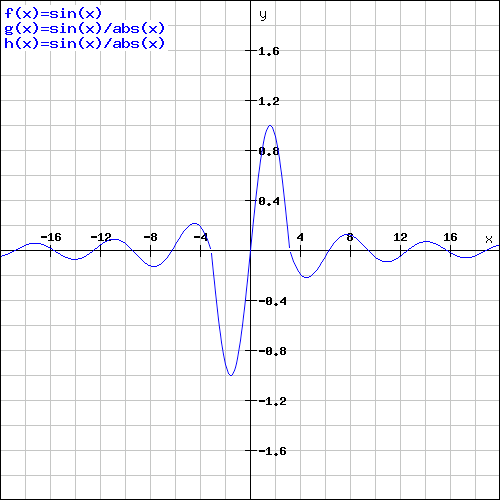
\includegraphics[width=6cm,height=6cm]{fig01.png} }}
    \subfloat[Derivative]{{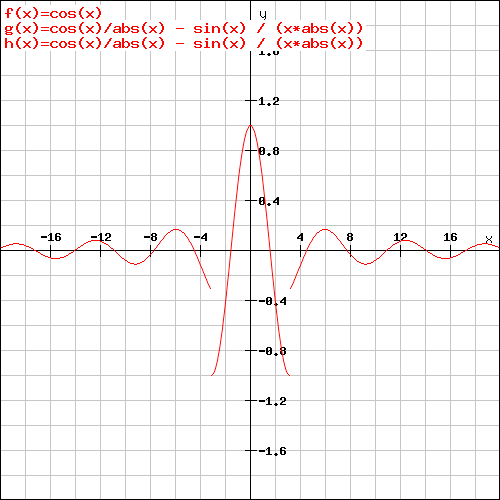
\includegraphics[width=6cm,height=6cm]{fig02.png} }}
    \caption{Fading sin activation function and its derivative.}
    \label{fig:fig02}
\end{figure}
\FloatBarrier
%
The problem with the sin fading function is that it has break points at -$\pi$ and +$\pi$.
%
\begin{equation}
\frac{d}{dx}f(x) = 
\left\{
	\begin{array}{ll}
		\cos(x) & \mbox{, } -\pi <= x <= +\pi \\
		\frac {\cos(x)} { |x| } - \frac{ \sin(x) }{ x |x| } & \mbox{, } +\pi < x < -\pi
	\end{array}
\right.
\end{equation}
%
The components of the function (Eq. 4) are differentiable functions (Eq. 5). This small inconvenience is not a problem when calculations are done with discrete number calculating computers. Representing real numbers in the computer memory is less accurate than the problems of analytic differentiability of the sin fading function. 
%
\section{Mobile Devices Distributed Computing}
%
The latest developments in mobile devices technology have made smartphones as the future computing and service access devices. Users expect to run computationally intensive applications on Smart Mobile Devices (SMDs) in the same way as powerful stationary computers [8]. Mobile Cloud Computing (MCC) is the latest practical solution for alleviating this incapability by extending the services and resources of computational clouds to SMDs on demand basis. In MCC, application offloading is ascertained as a software level solution for augmenting application processing capabilities of SMDs [8]. 

The proposed mobile client application is based on the capabilities of the Android Live Wallpaper [6]. On a regular basis a wallpaper service wakes up. At each wake up a single forecast is done. This forecast is then visualized as part of a wallpaper image. The wake up finishes a single ANN training epoche. The forecasting model is organized as a three-layers MLP instantiated as Encog framework Java object. Local ANN gradient based training is organized as resilient backpropagation which is provided by Encog framework. Training examples are generated from time series by dividing the values in a lag frame (values in the past) and lead frame (values in the future). In this way ANN tries to learn lag and lead patterns. All input data are normalized in the range of the used activation function (in this case -1 and +1, as shown in Fig. 1). Different instances of the ANN weights are presented as GA chromosomes. The error of ANN forecasts is used as fitness function in the local GA. On the side of the mobile client GA is represented as Java objects provided by Apache Commons Math Genetic Algorithms framework. In order for ANN training to be continuous and to be independent from Internet network connection, all ANN training examples are stored in a local SQLite database. The communication with the remote server is done only when there is better local solution. The information exchange between the client and the server is organized as HTTP sessions. All data exchanges are packaged as JSON messages. On the server side there is a PHP/MySQL based application which is described in [2]. 
%
\section{Experiments and Results}
%
All experiments are done with Encog framework by using Java programming language [9]. MLP neural network  (256-64-10 topology) is trained with examples of handwritten digits. Data set consists of 1593 handwritten digits from around 80 persons were scanned, stretched in a rectangular box 16x16 in a gray scale of 256 values [10]. Experiments are done on a single CPU core with the following parameters of the machine: Intel Core i7-4790 - 3.6GHz - 4 cores - 8 threads, 8GB RAM, Microsoft Windows 10, Encog Core v3.3.0 - Java Version, Java 8 Update 112 (64bit). 
%
\begin{figure}
    \centering
    \subfloat[MLP Error]{{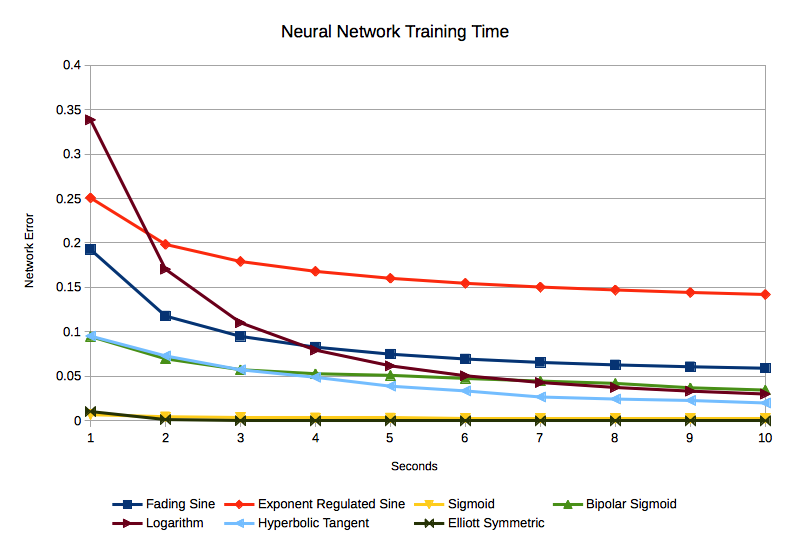
\includegraphics[width=6cm,height=6cm]{fig05.png} }}
    \subfloat[Training Epochs]{{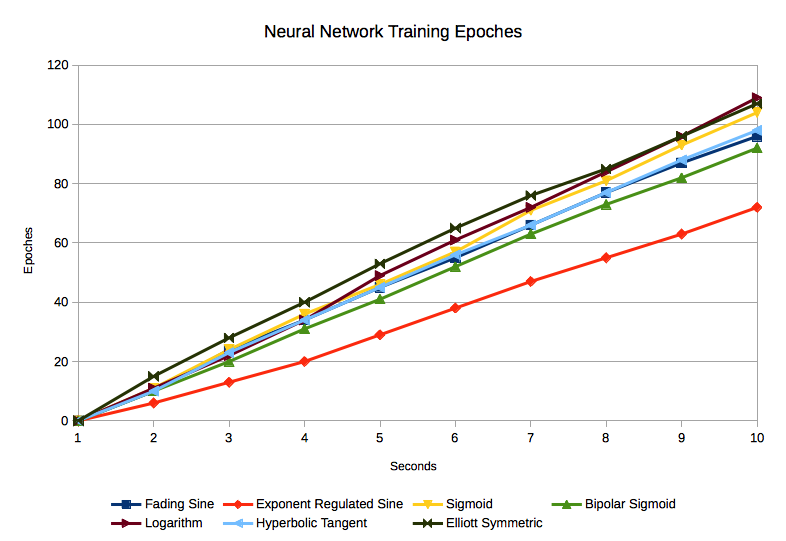
\includegraphics[width=6cm,height=6cm]{fig06.png} }}
    \caption{Activation functions efficiency.}
    \label{fig:fig02}
\end{figure}
\FloatBarrier
%
Comparison is done between seven activation functions - Fading Sin, Exponent Regulated Sin, Sigmoid, Bipolar Sigmoid, Logarithm, Hyperbolic Tangent, Elliott Symmetric. As it is shown in Fig. 3, between 70 and 110 training epoche are done for 10 seconds of training. The performance of exponent regulated sine is slower than the performance of fading sine. The network error for both functions decreases slower than the others, which is very logical because each neuron is limited in the activation signal which can be handled. This limitation gives better responsibilities separation between the neurons in each layer. 
%
\section{Conclusions}
%
Even though GA based ANN training is slower than back propagation, when it is implemented as simultaneous computations in a distributed environment it can be efficient enough for practical use. Because modern mobile devices are used on a 24/7 basis to use them as distributed computing network is very cost effective if the approach is based on donated computational power. As further development it will be interesting if mobile devices distributed computing is combined with supercomputers. The central node will be able to provide access to a super computer. Such hybrid infrastructure can provide interesting research and industrial challenges. Another very interesting direction of further development is the capabilities of Android widgets. The client side calculations are possible to be done in a widget instead of a wallpaper. Android widgets are interactive components in the graphical user interface. Such computational widget can be used for user voting or even user's guess for the future forecast. The collection of human opinion will transfer this software solution into the human-computer based distributed computing. 
%
\section*{Acknowledgements}
%
This work was supported by private funding of Velbazhd Software LLC.
%
% ---- Bibliography ----
%
\begin{thebibliography}{}
%
\bibitem[1] {bal:zan:1}
Balabanov, T., Zankinski, I., Barova, M.:
Strategy for Individuals Distribution by Incident Nodes Participation in Star Topology of Distributed Evolutionary Algorithms.
Cybernetics and Information Technologies, Sofia, Bulgaria, vol. 16, no. 1, 80--88  (2016)
%
\bibitem[2] {bal:dob:1}
Balabanov, T., Zankinski, I., Dobrinkova, D.:
Time Series Prediction by Artificial Neural Networks and Differential Evolution in Distributed Environment.
International Conference on Large-Scale Scientific Computing, Sozopol, Bulgaria, Lecture Notes in Computer Science, vol. 7116, no. 1, 198--205  (2011)
%
\bibitem[3] {bal:1}
Balabanov, T.:
Heuristic Forecasting Approaches in Distributed Environment (in Bulgarian).
Proceedings of Anniversary Scientific Conference 40 Years Department of Industrial Automation, UCTM, Sofia, Bulgaria, 163--166 (2011)
%
\bibitem[4] {bal:2}
Balabanov, T.:
Distributed evolutional model for music composition by human-computer interaction.
Proceedings of International Scientific Conference UniTech15, University publishing house V. Aprilov, Gabrovo, Bulgaria, vol. 2, 389--392 (2015)
%
\bibitem[5] {bal:3}
Balabanov, T.:
Avoiding Local Optimums in Distributed Population based Heuristic Algorithms (in Bulgarian).
Proceedings of XXIII International Symposium Management of energy, industrial and environmental systems, John Atanasoff Union of Automation and Informatics, Sofia, Bulgaria, 83--86 (2015)
%
\bibitem[6] {bal:zan:2}
Balabanov, T., Zankinski, I., Barova, M.:
VitoshaTrade Distributed Computing Android Wallpaper.
https://github.com/TodorBalabanov/VitDisComp Sofia, Bulgaria  (2017)
%
\bibitem[7] {kar:veh:1}
Karlik, B, Vehbi, A.:
Performance Analysis of Various Activation Functions in Generalized MLP Architectures of Neural Networks.
International Journal of Artificial Intelligence And Expert Systems (IJAE), vol. 1, no. 4, 111--122 (2011) 
%
\bibitem[8] {shi:gan:1}
Shiraz, M., Gani, A., Khokhar, R., Buyya, R.:
A Review on Distributed Application Processing Frameworks in Smart Mobile Devices for Mobile Cloud Computing.
IEEE Communications Surveys \& Tutorials, vol. 15, no. 3, 1294--1313 (2013) 
%
\bibitem[9] {zan:1}
Zankinski, I.:
Encog digits classification resilient training example with sin activation functions.
https://github.com/iliyanzan/DigitsResilient Sofia, Bulgaria  (2017)
%
\bibitem[10] {bus:tez:1}
Buscema, M., Terzi, S.:
Semeion Handwritten Digit Data Set.
Center for Machine Learning and Intelligent Systems, http://archive.ics.uci.edu/ml/datasets/Semeion+Handwritten+Digit California, USA  (2009)
%
\end{thebibliography}
\end{document}
